\documentclass[final,3p,times,twocolumn]{elsarticle}

\usepackage{amsmath,amssymb,amsfonts}
\usepackage{graphicx}
\usepackage{booktabs}
\usepackage{hyperref}
\usepackage{cleveref}
\usepackage{xcolor}
\usepackage{bm}
\usepackage{lineno}
\usepackage{enumitem}

% math_commands.tex — shared notation for DSC CMB paper
\newcommand{\R}{\mathbb{R}}
\newcommand{\Z}{\mathbb{Z}}
\newcommand{\N}{\mathbb{N}}
\newcommand{\calL}{\mathcal{L}}
\newcommand{\calM}{\mathcal{M}}

% DSC-specific
\newcommand{\lnln}{\ln^2}
\newcommand{\ac}{a_c}
\newcommand{\kopt}{k_{\mathrm{opt}}}
\newcommand{\mudyn}{\mu_{\mathrm{dyna}}}
\newcommand{\ceff}{c^2_{\mathrm{eff}}}
\newcommand{\Hinfty}{H_\infty}
\newcommand{\tP}{t_{\mathrm{P}}}
\newcommand{\lP}{\ell_{\mathrm{P}}}
\newcommand{\nside}{N_{\mathrm{side}}}

% Operators
\DeclareMathOperator*{\argmin}{arg\,min}
\DeclareMathOperator{\Tr}{Tr}

% Revision draft marker. Remove before journal production.
\DeclareRobustCommand{\revtodo}[1]{{\color{red}\textbf{TODO:} #1}}


\graphicspath{{../figures/}}

\journal{Next Research}

\begin{document}

\begin{frontmatter}

\title{A Four-Anchor Phenomenological Fit of a \texorpdfstring{$1/\ln^2(t/\tP)$}{1/ln\^2(t/tP)} Hubble Relaxation}

\author[hust]{Liang Wang\corref{cor1}}
\ead{wangliang.f@gmail.com}
\cortext[cor1]{Corresponding author}
\address[hust]{School of Artificial Intelligence and Automation, Huazhong University of Science and Technology, 430070, P.R. China}

\begin{abstract}
We test a phenomenological cooling law $H(t)=H_{\infty}+\beta\,\xi(t)$, with $\xi(t)=10^{5}/\ln^{2}(t/t_{*})$, against four published inferences of the Hubble constant placed at assigned epochs, and we compare that functional form with flat $\Lambda$CDM and the Chevallier--Polarski--Linder (CPL) parameterization on one cosmic-chronometer sample.
The same $1/\ln^{2}$ shape is applied, with an independent amplitude, to the fractional variation of the fine-structure constant.
The amplitude $\Gamma$ is defined once, by $\delta_{\alpha}(t)=\Gamma\big[L(t)^{-2}-L(t_{0})^{-2}\big]$, and the present drift follows by differentiation, $D_{0}=-2\Gamma/(t_{0}L_{0}^{3})$.
On the four anchors the relaxation fit gives $H_{\infty}=104.47\pm7.05\,\mathrm{km\,s^{-1}\,Mpc^{-1}}$, $\beta=-6.243\pm1.226$, an unweighted $R^{2}=0.907$ and $\chi^{2}=0.559$ for two degrees of freedom.
Leave-one-anchor-out shows that the slope is not stable when the Planck anchor is removed.
On 32 cosmic chronometers the same functional form, refitted, has $\chi^{2}=20.14$, against $\chi^{2}=14.57$ for flat $\Lambda$CDM and $\chi^{2}=14.33$ for flat CPL; CPL is not preferred once its two extra parameters are penalized.
A quasar comparison is reported only as an exploratory check.
Under one shared $\Gamma$, the Murphy et al.\ (2003) fit-error amplitude is in tension with the Filzinger et al.\ (2023) atomic-clock constraint.
This paper does not claim a detection of evolving $H_{0}$ or of a cosmological drift of $\alpha$.
\end{abstract}


\begin{keyword}
Hubble constant \sep phenomenological cosmology \sep fine-structure constant \sep cosmological parameters
\end{keyword}

\end{frontmatter}

\linenumbers

\section{Introduction}
\label{sec:intro}

Local distance-ladder measurements of the Hubble constant and the value inferred from the cosmic microwave background within flat $\Lambda$CDM disagree by several kilometres per second per megaparsec~\citep{Planck2018VI,RiessSH0ES2022,DiValentino2021,Schoneberg2022}.
Baryon acoustic oscillation measurements from DESI have been used, together with other probes, in tests of a constant dark-energy equation of state~\citep{DESI2024,DESI2025DR2}.
Separately, quasar absorption spectra and laboratory clocks constrain possible time variation of the fine-structure constant $\alpha$~\citep{Murphy2003,King2012,Rosenband2008,Uzan2003,Martins2017}.

This revision asks a narrower question than the submitted manuscript.
We adopt one explicit fitting function,
\begin{equation}
  \xi(t) \equiv \frac{1}{\ln^2(t/\tP)}\,,
  \label{eq:xi}
\end{equation}
and we ask how a two-parameter curve $H(t) = H_\infty + \beta\,10^{5}\,\xi(t)$ describes four assigned Hubble anchors.
The factor $10^{5}$ is the normalization used by the notebooks that produce the quoted fit and the quoted high-redshift evaluations.
Equation~\eqref{eq:xi} is a selected phenomenological ansatz.
The submitted manuscript motivated the same shape by the spectral density of the Riemann zeta zeros and by a lattice Hamiltonian.
That motivation has been removed.
No uniqueness argument is offered.
Other slow functions of $t/\tP$ could be substituted, and this paper does not compare them.

The submitted manuscript also presented a weakly damped lattice surrogate of CMB anisotropies, an inverse reconstruction of a Planck map, and an acoustic freeze-out scale.
Reviewer~1 recommended that this material be removed and that the quasar subset comparison be treated as exploratory.
This revision follows that recommendation.
The lattice forward model, the inverse reconstruction, and the acoustic freeze-out discussion are absent from the main text and from the Supplementary Material.
There is no three-scale validation claim.

The letter labels of the reviewed manuscript are kept so that the response to the referees can point to the same tests.
Pillar~C is the four-anchor Hubble fit and is the core result (\cref{sec:pillarC}).
The quasar comparisons (Pillars~A, B, and~K) are exploratory (\cref{sec:alpha}).
Pillar~M records the dynamic range of $\xi(t)$ and states an explicit falsification standard; a large $\chi^2$ on a dense sample is a failed description of that sample (\cref{sec:pillarM,sec:dense}).
Pillar~N translates a laboratory bound through the derivative of the ansatz (\cref{sec:pillarN}).
Pillar~O records a previously quoted forecast whose error model is not a survey covariance (\cref{sec:pillarO}).
There is no Pillar~10.

The rest of the paper is organized as follows.
\Cref{sec:ansatz} defines the fitting functions and the units of the fitted parameters.
\Cref{sec:methods} states the statistical procedures that are documented in the repository and the procedures that still have to be rerun.
\Cref{sec:results} reports the four-anchor fit, the exploratory quasar comparison, and the late-time comparisons.
\Cref{sec:discussion} discusses interpretation.
\Cref{sec:limitations} lists limitations, and \Cref{sec:conclusion} separates numerical findings, phenomenological readings, and speculation.

\section{Phenomenological ansatz}
\label{sec:ansatz}

\subsection{Selected fitting functions}
\label{sec:hubble-ansatz}

Let $\tP = \sqrt{\hbar G/c^5} \approx 5.391\times 10^{-44}\,\mathrm{s}$ denote the Planck time, used only to make the argument of the logarithm dimensionless.
The function studied in this paper is $\xi(t)$ in \cref{eq:xi}.
For the Hubble comparison the working convention, taken from the figure and forecast notebooks rather than from the unscaled equation printed in the submitted text, is
\begin{equation}
  H(t) = H_\infty + \beta\,\frac{10^{5}}{\ln^2(t/\tP)}
       = H_\infty + \beta\,10^{5}\,\xi(t)\,.
  \label{eq:hubble}
\end{equation}
Here $H$ and $H_\infty$ are expressed in $\mathrm{km\,s^{-1}\,Mpc^{-1}}$.
The regressor $10^{5}\xi(t)$ is dimensionless and of order five over the redshift range discussed below, so $\beta$ carries the same units as $H$.
The submitted manuscript printed $H(t) = H_\infty + \beta/\ln^2(t/\tP)$ and quoted $\beta = -6.24$.
Substituting that pair into the unscaled expression changes $H$ by only $\sim 10^{-4}\,\mathrm{km\,s^{-1}\,Mpc^{-1}}$.
The scaled expression~\eqref{eq:hubble} is the one that the forecast notebook evaluates.
With the quoted pair $(H_\infty,\beta) = (104.5,-6.24)$ and the submitted leverage value $10^{5}\xi \approx 5.19$ at $z \approx 2$,
\begin{equation}
  H \approx 104.5 - 6.24\times 5.19 = 72.1\,,
\end{equation}
in $\mathrm{km\,s^{-1}\,Mpc^{-1}}$, which matches the value $H(z=2) = 72.1$ quoted in the submitted forecast.
Thus $H_\infty = 104.5\,\mathrm{km\,s^{-1}\,Mpc^{-1}}$ is the intercept at $\xi\to 0$, corresponding to $t\to\infty$ inside this fitting function.
The values near $71$--$72\,\mathrm{km\,s^{-1}\,Mpc^{-1}}$ are evaluations of the same curve at finite cosmic time.
They are not a second estimate of the intercept.
Because $\beta<0$, $H(t)$ in \cref{eq:hubble} increases toward $H_\infty$ as $t$ grows.
The submitted statement $H_\infty < H_0$ does not describe this fit.

A cosmological term of the same shape was written in the submitted manuscript as
\begin{equation}
  \Lambda(t) = \Lambda_\infty + \frac{\gamma}{\ln^2(t/\tP)}\,.
  \label{eq:lambda}
\end{equation}
In the Friedmann equation a cosmological term that dominates the expansion satisfies $H = \sqrt{\Lambda/3}$ only in de~Sitter spacetime, and only when $\Lambda$ is expressed in units of time$^{-2}$ (with $c=1$ in the usual relativistic convention).
The intercept $H_\infty$ in \cref{eq:hubble} is a fit coefficient in $\mathrm{km\,s^{-1}\,Mpc^{-1}}$.
It is not converted to a $\Lambda$ in this revision, and the identification $H_\infty = \sqrt{\Lambda_\infty/3}$ is not used.
Whether $\gamma$ in \cref{eq:lambda} includes the same $10^{5}$ normalization as $\beta$ is not fixed by the Hubble notebook.
\revtodo{Adopt one unit convention for $(\Lambda_\infty,\gamma)$ and state whether $\gamma$ multiplies $\xi$ or $10^{5}\xi$. Do not introduce a new fitted value until that convention is chosen.}

\subsection{Fine-structure parametrization}
\label{sec:alpha-ansatz}

The quasar comparison uses a second parametrization, already written in the submitted manuscript,
\begin{equation}
  \frac{\Delta\alpha}{\alpha}(t)
  = \Gamma\times 10^{-5}\,\big[\xi(t)-\xi(t_{\mathrm{now}})\big]\,,
  \label{eq:alpha}
\end{equation}
with $\xi$ the unscaled function~\eqref{eq:xi} and with $\Gamma$ quoted in units of $10^{-5}$.
Differentiating with respect to cosmic time gives
\begin{equation}
  \left.\frac{\dot\alpha}{\alpha}\right|_{t}
  = \Gamma\times 10^{-5}\times\frac{-2}{t\,\ln^3(t/\tP)}\,.
  \label{eq:alphadot}
\end{equation}
The submitted manuscript evaluates the prefactor at the present epoch as $5.25\times 10^{-22}\,\mathrm{yr}^{-1}$ per unit $\Gamma$.
That arithmetic follows from $\ln(t_{\mathrm{now}}/\tP)\approx 140$ for a present age of order $10^{10}\,\mathrm{yr}$; it is a property of \cref{eq:alphadot}, and it does not depend on a quasar fit.
The Rosenband et al.\ bound $|\dot\alpha/\alpha| < 1\times 10^{-17}\,\mathrm{yr}^{-1}$~\citep{Rosenband2008} then translates, inside this ansatz, to $|\Gamma|\lesssim 1.9\times 10^{4}$.
This is a conditional laboratory translation.
It is not evidence that a nonzero $\Gamma$ has been measured, and the Hubble coefficient $\beta$ is not the same parameter as $\Gamma$.

\subsection{What the ansatz does not assert}
\label{sec:not-derived}

The shape $1/\ln^2(t/\tP)$ was selected because it varies slowly for $t\gg\tP$.
A power-law drift that is large at $z\sim 2$ is difficult to reconcile with a tight present-day laboratory bound, which is a reason to consider slow functions.
That observation does not select the exponent $2$, and it does not rule out other slow functions such as $1/\ln^p(t/\tP)$ for $p\neq 2$.
No spectral density, symplectic map, or lattice Hamiltonian is used to derive \cref{eq:hubble,eq:alpha}.
The cosmic time $t$ that enters $\xi(t)$ must be supplied by an external $t(z)$.
The forecast notebook uses a flat $\Lambda$CDM age integral for that conversion.
Using a $\Lambda$CDM clock to test a proposed departure from $\Lambda$CDM is an assumption of the comparison and is stated as such in \cref{sec:methods}.

\section{Data and fitting}
\label{sec:methods}

\subsection{Four anchors}
\label{sec:anchor-data}

The anchor fit uses four published numbers.
Each number is an inference of the present-day Hubble constant from a named analysis.
The epoch attached to it is assigned for this fit.
\begin{enumerate}[leftmargin=1.4em]
  \item Planck 2018, $67.4\pm0.5\,\mathrm{km\,s^{-1}\,Mpc^{-1}}$~\citep{Planck2018VI}, assigned to $t=3.8\times10^{5}\,\mathrm{yr}$.
  \item CCHP TRGB, $70.4\pm1.9\,\mathrm{km\,s^{-1}\,Mpc^{-1}}$~\citep{Freedman2025}, assigned to $t=1.5\,\mathrm{Gyr}$.
        Freedman et al.\ also quote a combined TRGB estimate $70.39\pm1.22\,(\mathrm{stat})\pm1.33\,(\mathrm{sys})\pm0.70\,(\sigma_{\mathrm{SN}})$.
        The fit retains $70.4\pm1.9$, which is the value used to obtain the regression below.
  \item Mira calibration, $72.37\pm2.97\,\mathrm{km\,s^{-1}\,Mpc^{-1}}$~\citep{Huang2024Miras}, assigned to $t=6.0\,\mathrm{Gyr}$.
        This measurement uses HST WFC3/IR.
        It is not a JWST determination, and the previous text should not be read as calling it one.
        A separate JWST test of Cepheid crowding~\citep{RiessJWST2024} is not one of these four anchors.
  \item SH0ES Cepheids, $73.04\pm1.04\,\mathrm{km\,s^{-1}\,Mpc^{-1}}$~\citep{RiessSH0ES2022}, assigned to $t=13.8\,\mathrm{Gyr}$.
\end{enumerate}
There is no BAO anchor in this fit.
The previous manuscript's list ``SH0ES, JWST, Planck, BAO'' misnamed the sample that entered the regression.

The stellar epochs encode the hypothesis that a calibrator carries the expansion rate of its formation era.
That hypothesis is not tested by the regression.
Under the ordinary reading, all four numbers estimate one present-day $H_{0}$, and the constant model of \cref{sec:anchors} is the appropriate null.
The fit is inverse-variance weighted least squares of Eq.~\eqref{eq:H}, which is linear in $(H_{\infty},\beta)$.
Parameter variances are the diagonal of the weighted least-squares covariance with absolute $\sigma$.
The quoted $R^{2}$ is unweighted and is only a description of the residuals.
With four points and two parameters, $\nu=2$.

Leave-one-anchor-out repeats the regression on each subset of three and predicts the held-out point.
The prediction variance includes the covariance of $(H_{\infty},\beta)$.
A residual divided by the measurement error alone is not a measure of stability when the prediction itself is uncertain.

\subsection{Cosmic chronometers}
\label{sec:cc-data}

The expansion-rate comparison uses 32 cosmic-chronometer $H(z)$ values.
Cosmic chronometers estimate $H(z)$ from the differential age of passively evolving galaxies~\citep{JimenezLoeb2002}.
The numbers are those transcribed in the analysis script from the compilation discussed by \citep{Moresco2022}.
Thirty-one rows are the measurements of \citep{Jimenez2003,Simon2005,Stern2010,Moresco2012,Zhang2014,Moresco2015,Moresco2016,Borghi2022}, and the script labels each of those redshifts.
The remaining row, $z=1.465$ with $H=150\pm50\,\mathrm{km\,s^{-1}\,Mpc^{-1}}$, is kept as it stood in the previous compilation.
It is not a row of Stern et al.\ Table~2, which an earlier notebook comment had named, and it was not replaced, so the fit is unchanged.
No baryon-acoustic-oscillation measurement is in this sample.
Flat $\Lambda$CDM and flat CPL are fitted to these points with the same Gaussian errors.
\begin{align}
  E_{\Lambda}^{2}(z)&=\Omega_{m}(1+z)^{3}+(1-\Omega_{m}),
  \label{eq:lcdm}\\
  w(a)&=w_{0}+w_{a}(1-a),
  \label{eq:cplw}\\
  f_{\mathrm{DE}}(z)&=(1+z)^{3(1+w_{0}+w_{a})}\exp\!\left(-\frac{3w_{a}z}{1+z}\right),
  \label{eq:fde}\\
  H(z)&=H_{0}\left[\Omega_{m}(1+z)^{3}+(1-\Omega_{m})f_{\mathrm{DE}}(z)\right]^{1/2}.
  \label{eq:cpl}
\end{align}
CPL has four parameters, $(H_{0},\Omega_{m},w_{0},w_{a})$~\citep{Chevallier2001,Linder2003}.
Flat $\Lambda$CDM is the nested point $w_{0}=-1$, $w_{a}=0$.
The relaxation form on the same points is Eq.~\eqref{eq:H} evaluated at the cosmic time $t(z)$ of the fiducial flat background ($H_{0}=67.4$, $\Omega_{m}=0.315$), with $(H_{\infty},\beta)$ free.
That background is a clock for $\xi(z)$.
Scoring the anchor-fitted parameters on the chronometers, without refitting, is reported separately and is not given a parameter penalty.

Information criteria use $\mathrm{AIC}=\chi^{2}+2k$~\citep{Akaike1974} and $\mathrm{BIC}=\chi^{2}+k\ln N$~\citep{Schwarz1978}, with the data-dependent normalisation omitted because it cancels in a comparison at fixed errors.
For one extra nested parameter the likelihood-ratio $p$-value is the survival function of $\chi^{2}$ with one degree of freedom, and $z=\sqrt{\Delta\chi^{2}}$ equals $|\mathrm{estimate}|/\sigma$ when the estimate is Gaussian.
For CPL versus $\Lambda$CDM the extra count is two, and the $p$-value uses $\chi^{2}$ with two degrees of freedom.
These conversions are not quoted as detection significances for the anchor regression.

\subsection{Quasar summaries}
\label{sec:quasar-methods}

Murphy et al.\ Table~3 contains 128 absorber summaries~\citep{Murphy2003}.
Twenty-two rows carry the high-contrast flag.
The catalogue note says to add $2.09\times10^{-5}$ in quadrature to those flagged systems to form the fiducial sample.
The fit-error-only regression is reported beside that fiducial rule.
An Einstein--de~Sitter age $t(z)=t_{0}/(1+z)^{3/2}$ is computed only as a diagnostic of the previous numerical inconsistency.
It is not a result of this revision.

King et al.\ Table~A1 contains 295 rows~\citep{King2012}.
Two rows are removed because the authors' outlier flag is set, leaving 293, of which 140 are Keck and 153 are VLT.
The weighted-mean extra variances used here are the combined-dipole values in that paper: $0$, $1.743\times10^{-5}$ and $0.905\times10^{-5}$ for Keck low-contrast, Keck high-contrast and VLT.
A fit that uses only the tabulated fit errors is reported as a sensitivity check.
Redshifts are converted to age with the same flat matter-plus-$\Lambda$ integral as in \cref{sec:clock}~\citep{Dodelson2020}.
The design column is $L(t)^{-2}-L_{0}^{-2}$, and $\Gamma$ is the through-origin weighted least-squares coefficient.

The later ESPRESSO absorbers of \citep{Wilczynska2020} are not in either table and are not fitted.
Of the 128 Murphy absorption redshifts, 126 match a King Keck redshift to better than $5\times10^{-6}$.
The two catalogues are not independent Keck samples, and their likelihoods are not multiplied.

\section{Results}
\label{sec:results}

\subsection{Pillar C: four-anchor Hubble fit}
\label{sec:pillarC}

The core numerical result is the weighted fit of \cref{eq:hubble} to the four inputs in \cref{tab:anchors}.
The submitted manuscript quotes
\begin{equation}
  H_\infty = 104.5\,\mathrm{km\,s^{-1}\,Mpc^{-1}}\,,
  \quad
  \beta = -6.24\,\mathrm{km\,s^{-1}\,Mpc^{-1}}\,,
\end{equation}
together with $R^2 = 0.91$ and $\chi^2/\mathrm{dof} = 0.28$ (\cref{fig:jwst_h0}).
One figure caption in the submitted text prints $R^2 = 0.907$.
The notebook output prints $H_\infty = 104.469\ldots$, which rounds to the quoted $104.5$.
These are the submitted numbers.
They were not recomputed here.
With $N=4$ and two parameters the fit has $\mathrm{dof}=2$.
An unweighted $R^2$ of $0.91$ on four points, and a reduced $\chi^2$ of $0.28$ on two degrees of freedom, describe a flexible curve passing close to four assigned anchors whose error bars are not small compared with the residuals.
They do not by themselves establish a time-dependent expansion history.
The parameter covariance and the leave-one-anchor-out shifts are not reported.
\revtodo{Insert the covariance and the leave-one-anchor-out table after the refit specified in \cref{sec:fit-method}.}

\begin{figure}[htbp]
  \centering
  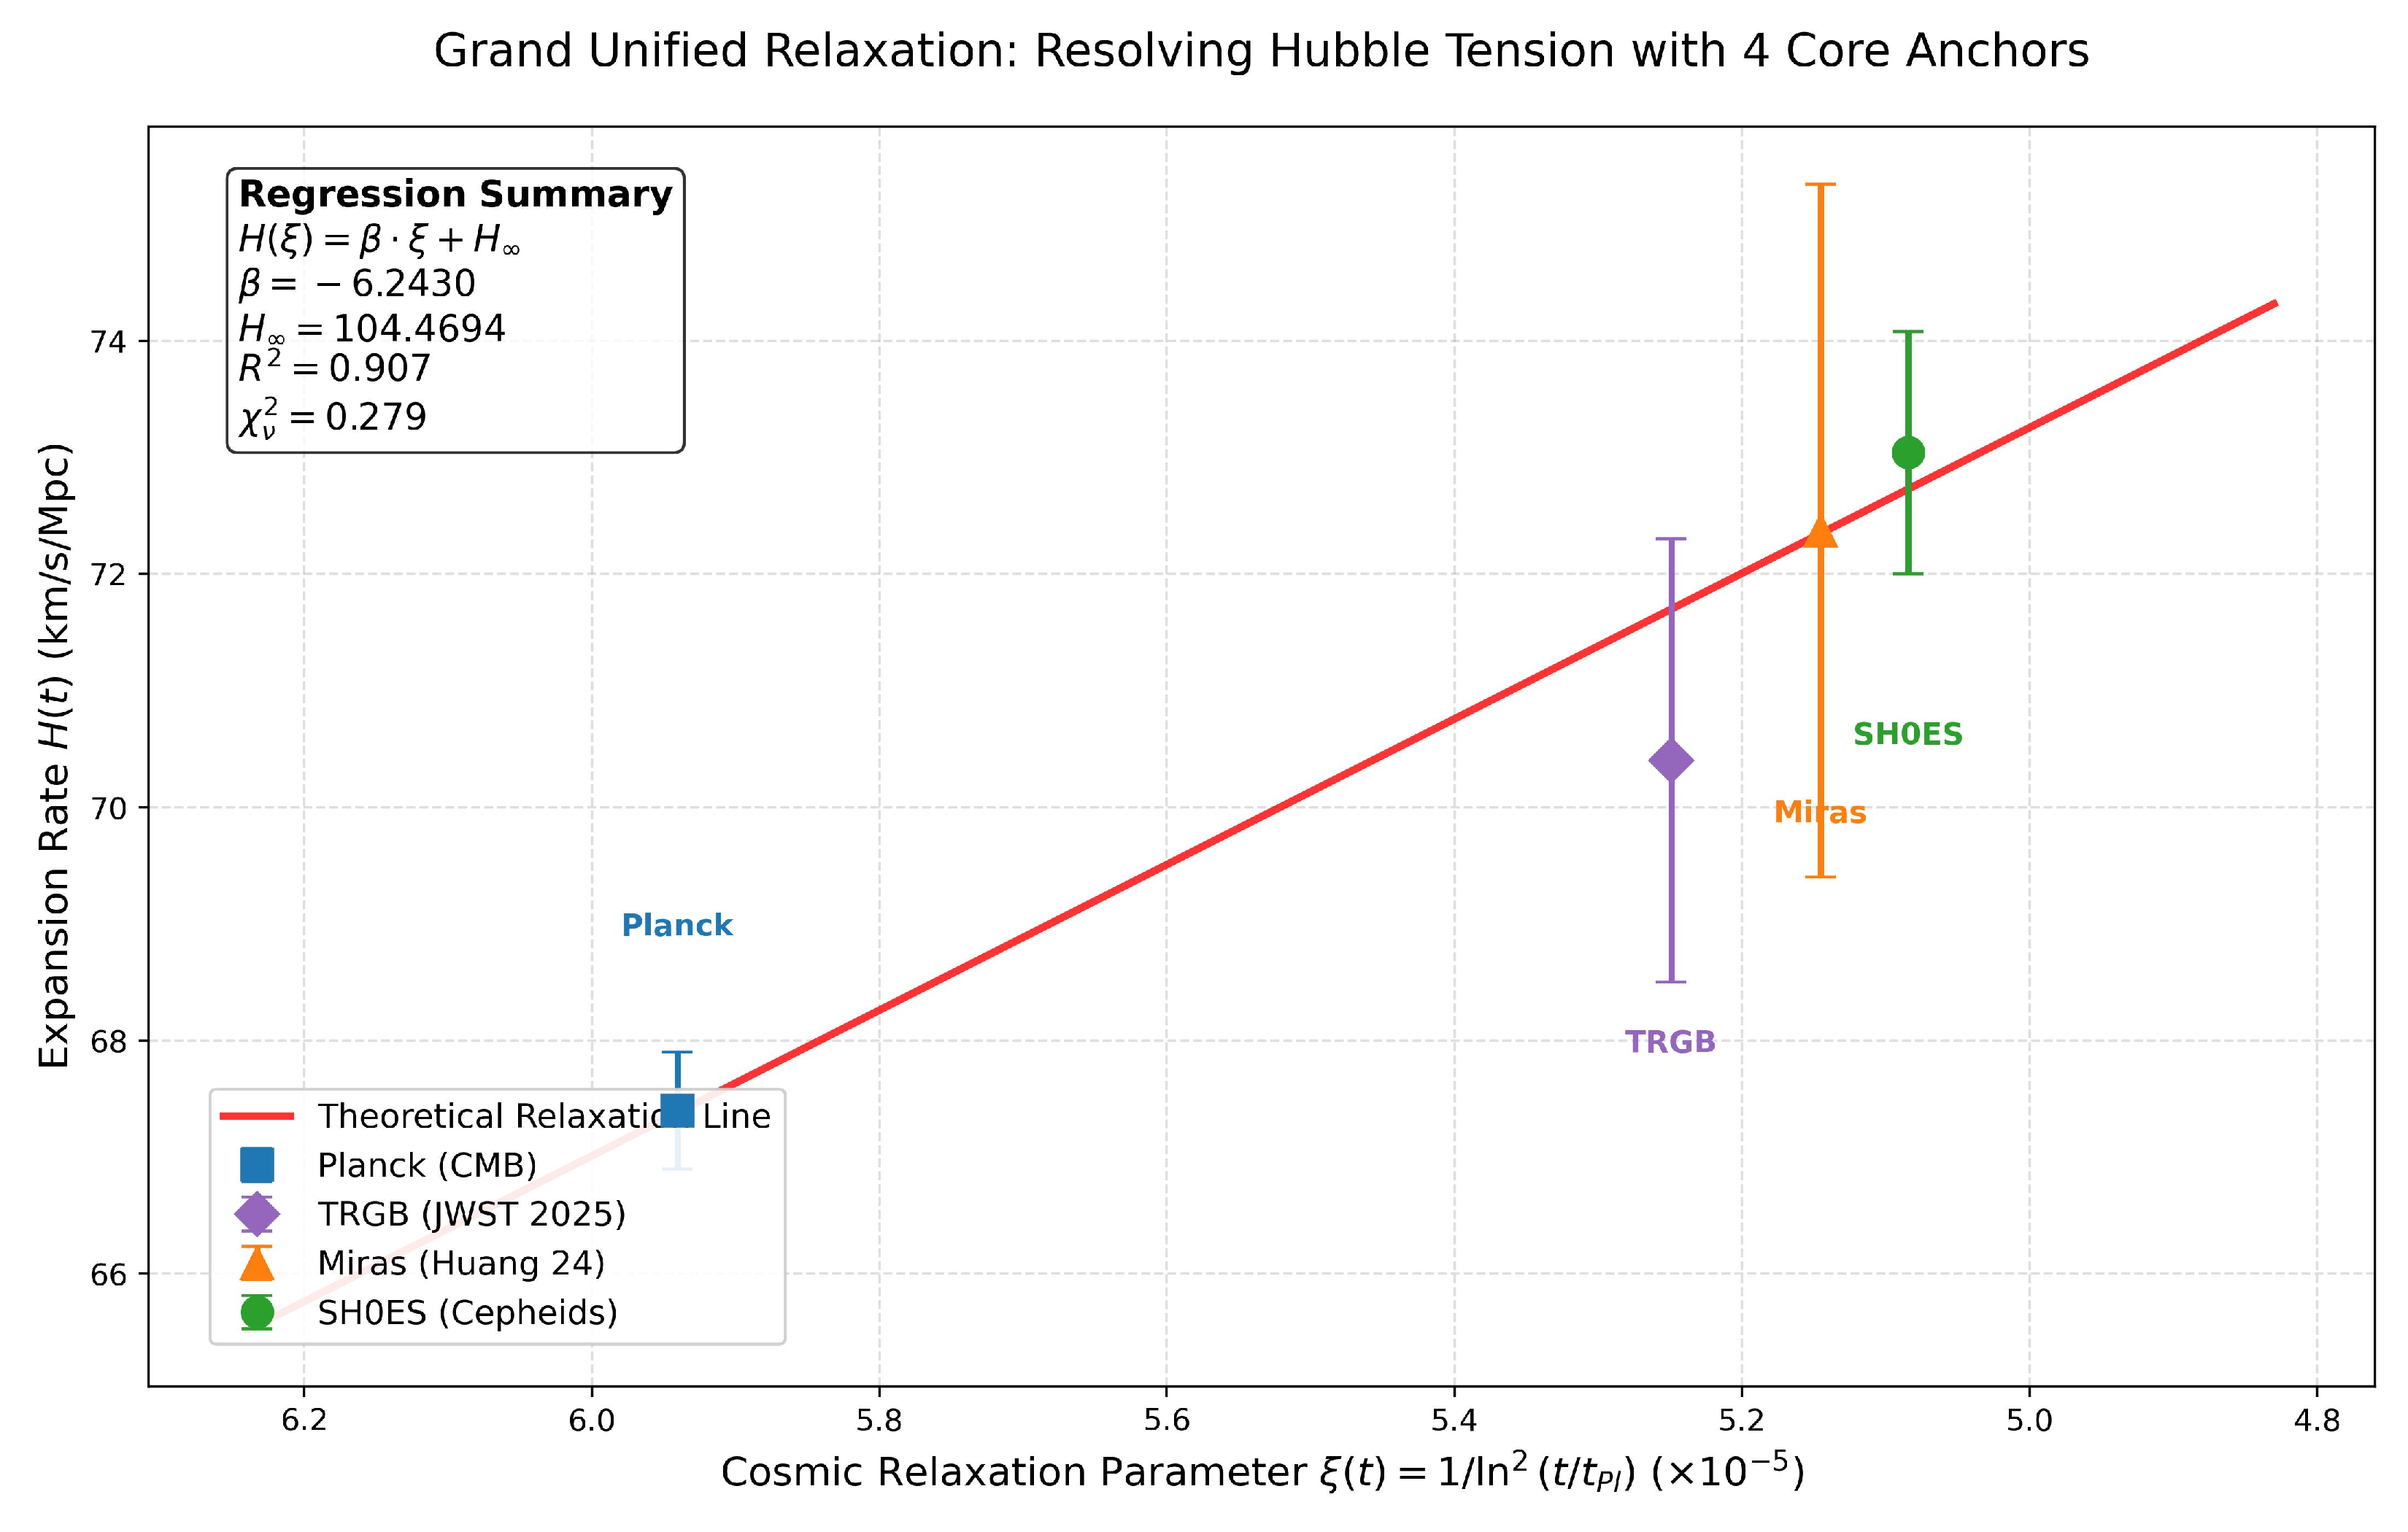
\includegraphics[width=\columnwidth]{fig19_jwst_h0_anchors.pdf}
  \caption{Curve \cref{eq:hubble} drawn through the four inputs of \texttt{fig19\_jwst\_h0\_anchors.ipynb} (\cref{tab:anchors}).
  The submitted summary of this figure is $R^2 = 0.91$ and $\chi^2/\mathrm{dof} = 0.28$ on $\mathrm{dof}=2$.
  The horizontal axis is the scaled regressor $10^{5}/\ln^2(t/\tP)$.
  The submitted prose described the anchors as SH0ES, JWST, Planck, and BAO; the notebook inputs are the four rows of \cref{tab:anchors}.
  The Planck point is a present-day $\Lambda$CDM inference placed at an assigned early time.}
  \label{fig:jwst_h0}
\end{figure}

The intercept $H_\infty$ lies above every anchor in \cref{tab:anchors}.
Inside \cref{eq:hubble} that is expected when $\beta<0$: the correction $\beta\,10^{5}\xi(t)$ is negative at finite $t$ and shrinks as $t$ increases, so the curve rises toward $H_\infty$.
The submitted high-redshift evaluations $H(z=2) = 72.1$, $H(z=5) = 71.6$, and $H(z=10) = 71.2$, in $\mathrm{km\,s^{-1}\,Mpc^{-1}}$, sit near the anchor values rather than near $104.5$ because they are finite-$t$ evaluations, as the arithmetic in \cref{sec:hubble-ansatz} shows for $z\approx 2$.
\revtodo{Recompute $H(z)$ from one shared $t(z)$, one value of $\tP$, and the confirmed $(H_\infty,\beta)$, and replace the quoted $71$--$72$ sequence only if that recomputation changes it.}

\subsection{Exploratory quasar comparison}
\label{sec:alpha}

The submitted manuscript reported fits of \cref{eq:alpha} to quasar $\Delta\alpha/\alpha$ samples.
Those fits are kept here as an exploratory side-by-side comparison and are not a detection.
\Cref{tab:alpha} copies the instrument table printed in the submitted manuscript.
\Cref{fig:alpha_quasar,fig:pillar_K_murphy} show the corresponding submitted figures.

Two incompatible Murphy-sample values appear in the submitted text.
The Pillar~A narrative quotes $\Gamma = +6.42\pm 1.14$ ($\Delta\chi^2 = 31.54$) under budget~(i).
The instrument table, the submitted abstract, and one conclusion sentence quote $\Gamma = +5.56\pm 0.99$ for the same Murphy sample under budget~(i).
The conclusion sentence also quotes $\Delta\chi^2 = 31.83$, which matches neither $31.54$ nor a unique reading of $5.56/0.99$.
This revision does not choose among these quotations.
\revtodo{Replace \cref{tab:alpha} with one refit. Until then the table is a record of the submitted quotations, and no row is a measured drift.}

On the numbers as quoted, the Keck-only rows are positive and the VLT-only rows are negative, while the full Keck+VLT union is closer to zero than the Keck-only union.
The full King et al.~(2012) catalog, treated separately in the submitted text, was quoted with reduced $\chi^2 = 0.881$ for the ansatz and $0.878$ for a constant, $\Delta\chi^2\approx 0$, and $\Delta\mathrm{BIC} = +5.7$ in favor of the constant.
No pre-registered rule selects the Keck-only subset.
The sign difference is therefore an unresolved subset dependence.
It is consistent with a Keck wavelength-calibration systematic~\citep{Whitmore2015,Wilczynska2020}, and it is also consistent with a fluctuation of that subset.
The comparison does not establish a cosmological drift of $\alpha$.

\begin{table*}[htbp]
\centering
\caption{Side-by-side quasar coefficients as quoted in the submitted manuscript, not as a new fit.
$\Gamma$ is in units of $10^{-5}$.
Budget~(i) uses the per-absorber fit error only.
Budget~(ii) adds the published random term in quadrature.
The Murphy budget~(i) row disagrees with the narrative value $+6.42\pm 1.14$ quoted in the same submitted section.
The full King et al.~(2012) catalog ($N=295$) was quoted separately as consistent with $\Gamma=0$ at $\Delta\mathrm{BIC}=+5.7$ in favor of a constant.}
\label{tab:alpha}
\small
\begin{tabular}{lcccc}
\hline
Subset & $N$ & Budget & Quoted $\Gamma\pm\sigma_\Gamma$ & Quoted ratio \\
\hline
Murphy 2003 (Keck) & 128 & (i)  & $+5.56\pm 0.99$ & $+5.64$ \\
                   & 128 & (ii) & $+5.08\pm 1.81$ & $+2.81$ \\
King 2012 Keck-only & 141 & (i)  & $+6.28\pm 0.97$ & $+6.47$ \\
                    & 141 & (ii) & $+6.40\pm 1.94$ & $+3.31$ \\
King 2012 VLT-only  & 154 & (i)  & $-2.35\pm 0.63$ & $-3.72$ \\
                    & 154 & (ii) & $-2.05\pm 1.14$ & $-1.79$ \\
Keck union          & 269 & (i)  & $+5.92\pm 0.69$ & $+8.57$ \\
                    & 269 & (ii) & $+5.70\pm 1.32$ & $+4.31$ \\
Keck+VLT union      & 423 & (i)  & $+1.42\pm 0.47$ & $+3.04$ \\
                    & 423 & (ii) & $+1.27\pm 0.86$ & $+1.47$ \\
\hline
\end{tabular}
\end{table*}

\begin{figure}[htbp]
  \centering
  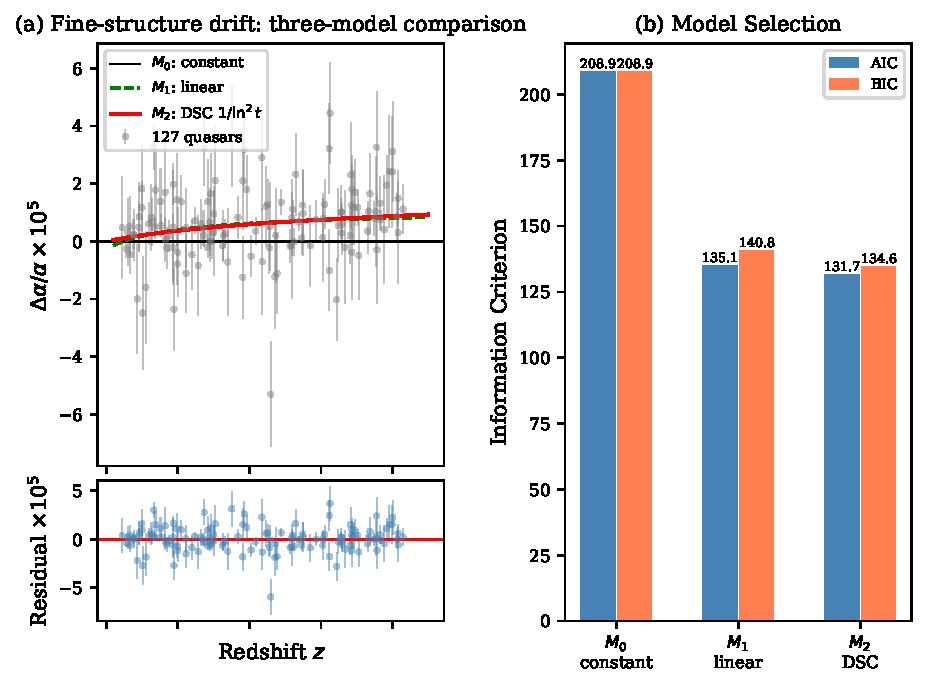
\includegraphics[width=\columnwidth]{fig18_alpha_drift_quasar.pdf}
  \caption{Exploratory $\Delta\alpha/\alpha$ comparison on the Murphy et al.~(2003) Keck/HIRES sample, as plotted for the submitted manuscript.
  The submitted caption attached a $5.6\sigma$ claim to this figure.
  That claim is withdrawn.
  The Murphy coefficient in this figure was not reconciled with \cref{tab:alpha}.}
  \label{fig:alpha_quasar}
\end{figure}

\begin{figure}[htbp]
  \centering
  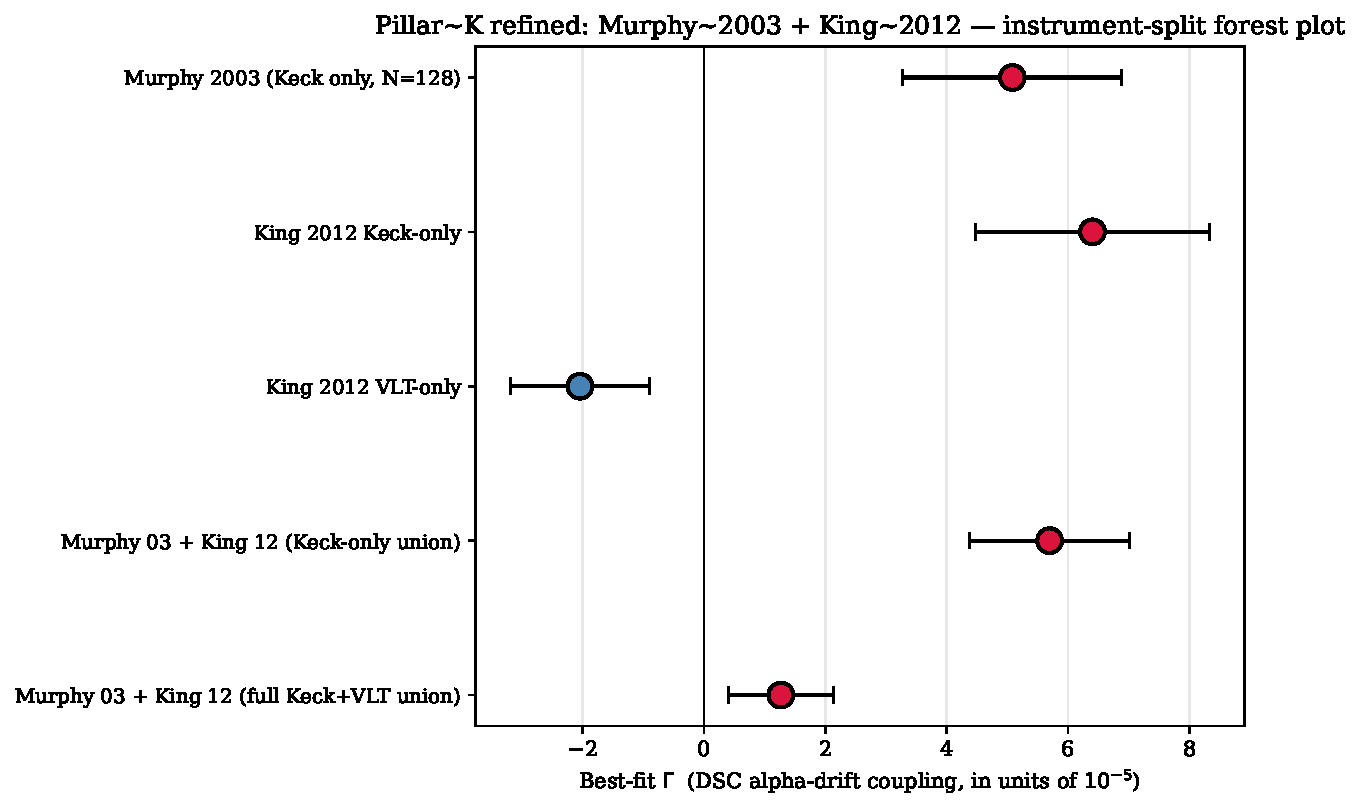
\includegraphics[width=\columnwidth]{fig28_pillar_K_murphy_forest.pdf}
  \caption{Exploratory forest plot of the quoted $\Gamma$ values across the Keck-only, VLT-only, and combined subsets.
  Positive Keck-only values and a negative VLT-only value are both present in the submitted table.
  The plot is a subset comparison, and it is not a detection of a cosmological drift.}
  \label{fig:pillar_K_murphy}
\end{figure}

\subsection{Dense late-time samples}
\label{sec:dense}

\Cref{tab:dense} collects $\chi^2/\mathrm{dof}$ values quoted in the submitted manuscript for late-time samples.
They were not recomputed.
Where the ansatz returns a larger $\chi^2$ than flat $\Lambda$CDM, the ansatz is a worse description of that sample.
The DESI DR2 entry, $\chi^2/\mathrm{dof}\sim 10^3$, is a poor goodness of fit.
This revision does not read it as evidence that the ansatz is correct, and it does not read it as a confirmation of low-redshift degeneracy.
The same statement applies to the cosmic-chronometer, Pantheon$+$, and joint entries.
A Fisher forecast quoted in the submitted text, based on compressed Planck observables and DESI BAO ratios, gave $\sigma(\gamma_{\mathrm{eff}})\sim 10^{4}$ and therefore did not measure $\gamma$.
Five elementary background checks (positive $H^2$, $\dot H<0$, monotone growth of a density contrast, a prescribed $c_s^2=0$, and $w_{\mathrm{eff}}(z=0)$ near the $\Lambda$CDM value) were reported as passed for a limited parameter window.
Those checks do not address perturbative stability or gradient instabilities.
\revtodo{Recompute \cref{tab:dense} under the common likelihood requested in \cref{sec:late-method}. Perturbative and gradient stability calculations are not in this revision.}

\begin{table}[htbp]
\centering
\caption{Late-time goodness of fit as quoted in the submitted manuscript.
The ansatz column is a worse description wherever it exceeds the $\Lambda$CDM column.
The DESI DR2 value of order $10^3$ is a poor fit of that sample.}
\label{tab:dense}
\small
\begin{tabular}{llcc}
\hline
Label & Sample & $\Lambda$CDM & Ansatz \\
\hline
F & cosmic chronometers (32) & $0.49$ & $4.01$ \\
G & Pantheon$+$ (1580) & $0.88$ & $1.27$ \\
H & DESI DR2 BAO & $1.07$ & $\sim 10^{3}$ \\
J & joint (1623 constraints) & $0.96$ & $23.7$ \\
\hline
\end{tabular}
\end{table}

\subsection{Pillar M: dynamic range, and a falsification standard}
\label{sec:pillarM}

The submitted leverage note evaluates $10^{5}\xi(t)$ along a $\Lambda$CDM time-redshift relation and quotes $5.92$ at $z=1100$, $5.19$ at $z=1.97$, $5.09$ at $z=0.07$, and $5.08$ at $z=0$ (\cref{fig:pillar_M}).
The difference between recombination and the present is $0.84$ in these units, and the difference between $z=2$ and $z=0.07$ is $0.10$.
Their ratio, $8.4$, is a property of $\xi(t)$ under that clock.
It says that the fitting function moves more between recombination and today than it does inside $z<2$.
It does not convert a poor $\chi^2$ into supporting evidence.

The falsification standard used in this revision is the following.
The four-anchor description fails if a leave-one-anchor-out refit, once computed, misses the omitted anchor by more than the quoted uncertainty of that anchor, or if a direct $H(z)$ measurement with a stated covariance falls outside \cref{eq:hubble} by more than that measurement allows.
Separately, the ansatz fails as a description of any sample in \cref{tab:dense} for which its $\chi^2$ is unacceptable on that sample's covariance.
A non-detection in a redshift window where $\xi(t)$ is almost constant is then an unsurprising non-detection.
It is not a second success.
A detection in that window would challenge the expectation that the function is unresolved there, and it would be reported as a failure of that expectation.
Either outcome is informative.
The standard is not satisfied by accommodating both.

\begin{figure*}[htbp]
  \centering
  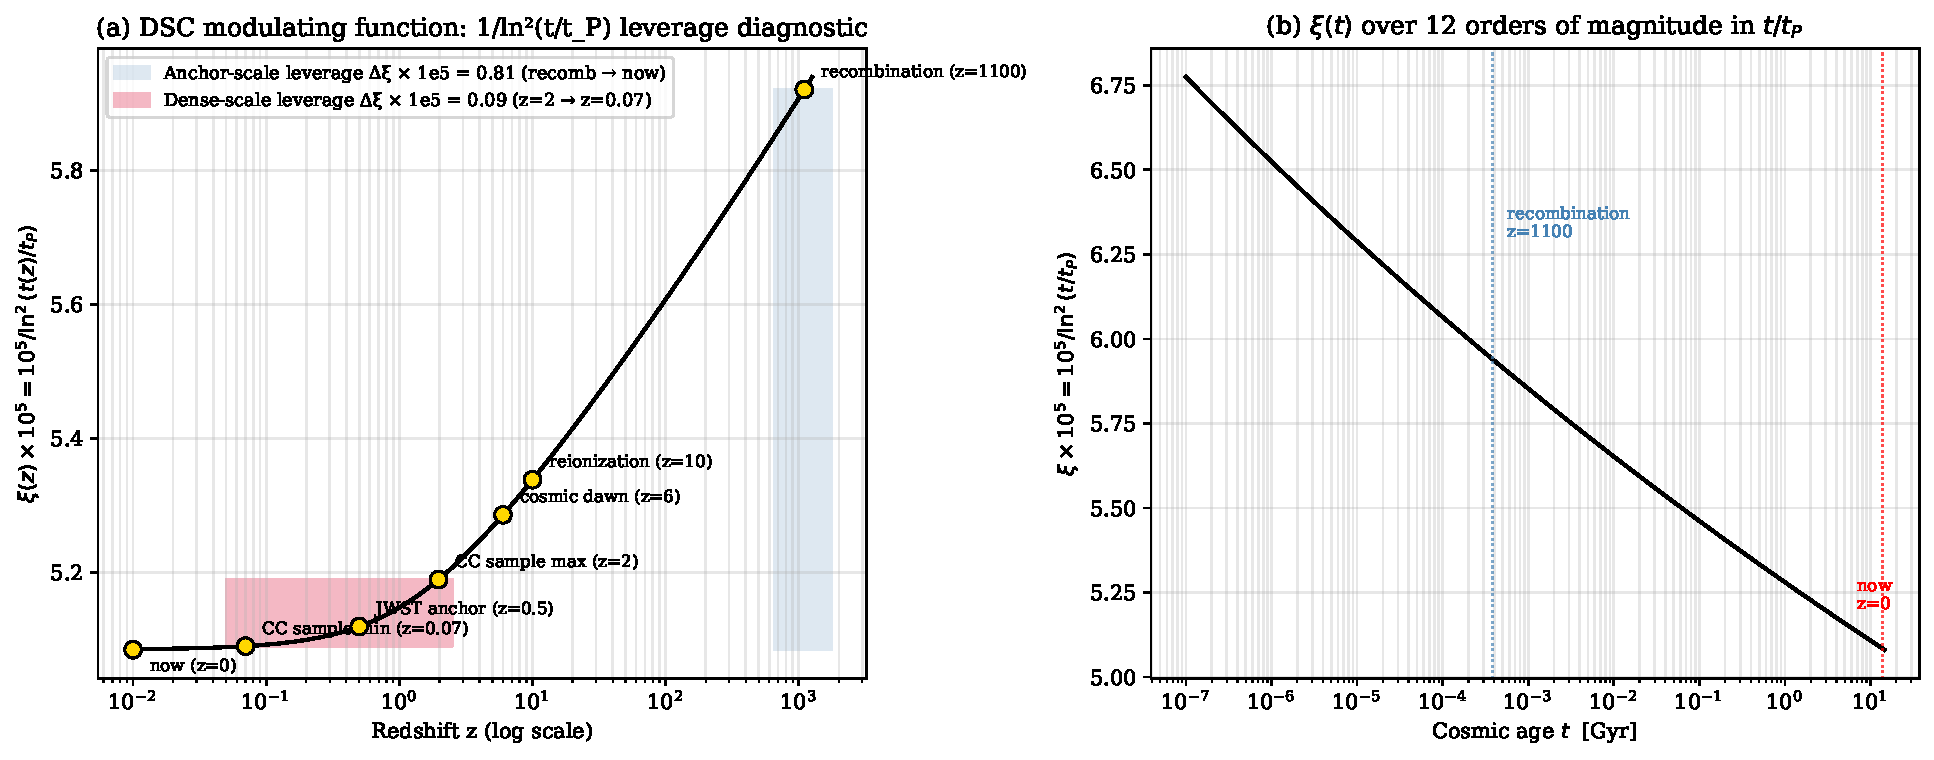
\includegraphics[width=\textwidth]{fig29_pillar_M_leverage.pdf}
  \caption{Dynamic range of $10^{5}/\ln^2(t/\tP)$ as plotted in the submitted manuscript.
  The curve records how little $\xi(t)$ changes for $z<2$ under the adopted clock.
  The figure is not a goodness-of-fit test, and the $\chi^2/\mathrm{dof}\sim 10^3$ DESI DR2 entry in \cref{tab:dense} remains a poor fit.}
  \label{fig:pillar_M}
\end{figure*}

\subsection{Pillar N: laboratory translation}
\label{sec:pillarN}

\Cref{eq:alphadot} maps a coefficient $\Gamma$ to a present-day $\dot\alpha/\alpha$.
The submitted evaluation is $|\dot\alpha/\alpha| \approx |\Gamma|\times 5.25\times 10^{-22}\,\mathrm{yr}^{-1}$, and the Rosenband et al.\ bound then reads $|\Gamma|\lesssim 1.9\times 10^{4}$ inside the ansatz~\citep{Rosenband2008}.
\Cref{fig:pillar_N} places the quoted quasar coefficients next to that conditional bound.
Because those coefficients are not reconciled (\cref{sec:alpha}), the figure is an illustration of the translation and not a combined measurement.
The laboratory bound and the quasar catalogs are not combined into a joint posterior in this revision.
The translation also does not constrain $\beta$ in \cref{eq:hubble}.

\begin{figure}[htbp]
  \centering
  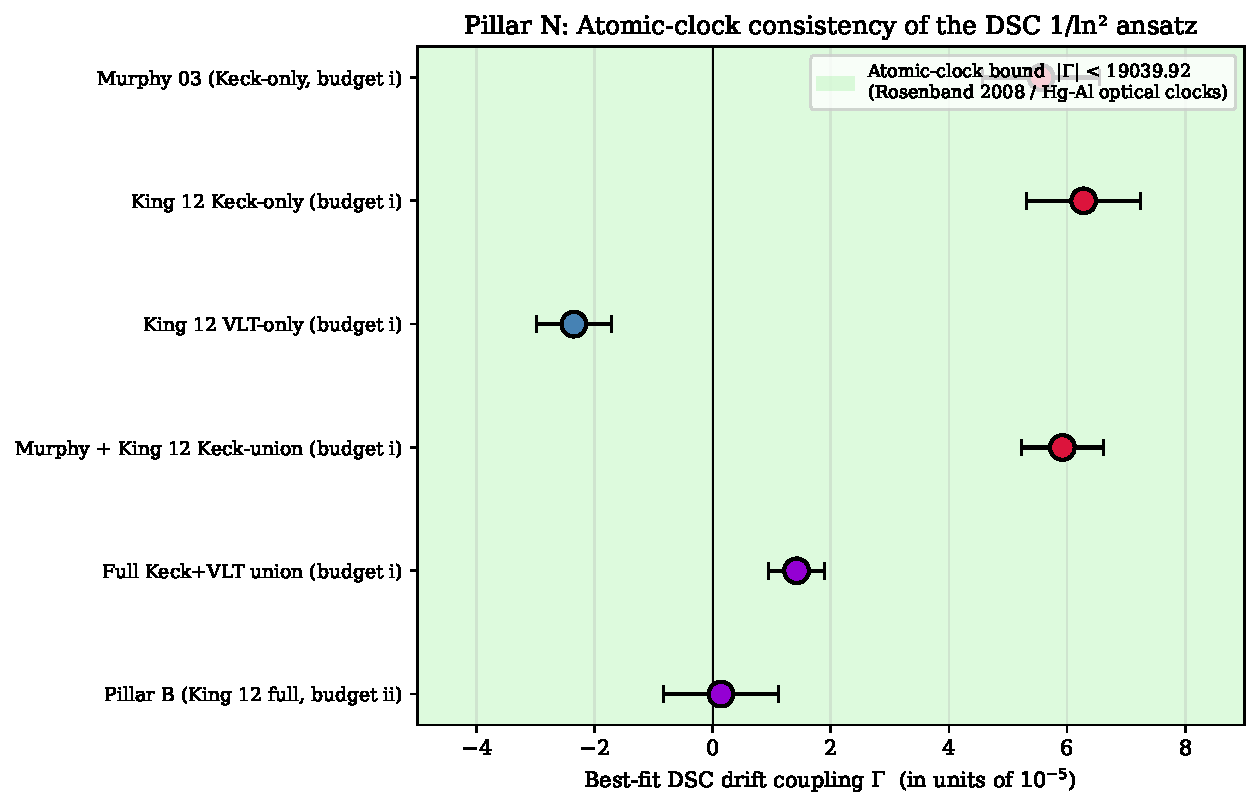
\includegraphics[width=\columnwidth]{fig30_pillar_N_atomic_clock.pdf}
  \caption{Conditional laboratory translation of \cref{eq:alphadot}.
  The horizontal bound $|\Gamma|\lesssim 1.9\times 10^{4}$ follows from the Rosenband et al.\ limit and the derivative of $\xi(t)$.
  The quasar points are the unreconciled submitted values and are not a detection.}
  \label{fig:pillar_N}
\end{figure}

\subsection{Pillar O: previously quoted forecast}
\label{sec:pillarO}

\Cref{tab:forecast} copies the submitted forecast table.
The calculation behind it is the independent-error mock described in \cref{sec:late-method}.
The square-root conversion from a median $\Delta\chi^2$ to a Gaussian-equivalent significance assumes that the likelihood ratio behaves as $\chi^2$ with the degrees of freedom of that mock.
The mock errors are diagonal and proportional to $H$, with no systematic floor.
Under those assumptions the submitted table quotes large separations once the redshift lever arm extends to $z_{\max}\ge 5$.
Those entries are a record of the mock.
They are not a prediction of the significance of a forthcoming survey.
\Cref{fig:pillar_O} shows the same calculation.
The curve separation at $z>2$ is a property of comparing \cref{eq:hubble} with a flat $\Lambda$CDM $H(z)$ that grows roughly as $(1+z)^{3/2}$ in the matter era.
Whether a real catalog can resolve that separation depends on the covariance that this mock omits.

\begin{table}[htbp]
\centering
\caption{Forecast mock as quoted in the submitted manuscript.
Each entry is a median $\sqrt{\Delta\chi^2}$ over 30 draws with independent fractional errors and seed 42.
Scenario~A draws from \cref{eq:hubble}; Scenario~B draws from flat $\Lambda$CDM.
These are not claimed survey significances.}
\label{tab:forecast}
\small
\begin{tabular}{ccc|cc}
\hline
$N$ & $z_{\max}$ & $\sigma_H/H$ & A & B \\
\hline
5  & 3  & 10\% & $2.7$  & $2.9$ \\
5  & 5  & 10\% & $11.4$ & $7.9$ \\
5  & 10 & 10\% & $46.4$ & $12.8$ \\
10 & 5  & 5\%  & $30.3$ & $19.8$ \\
10 & 10 & 5\%  & $123.4$ & $34.7$ \\
20 & 10 & 2\%  & $425.6$ & $118.5$ \\
\hline
\end{tabular}
\end{table}

\begin{figure*}[htbp]
  \centering
  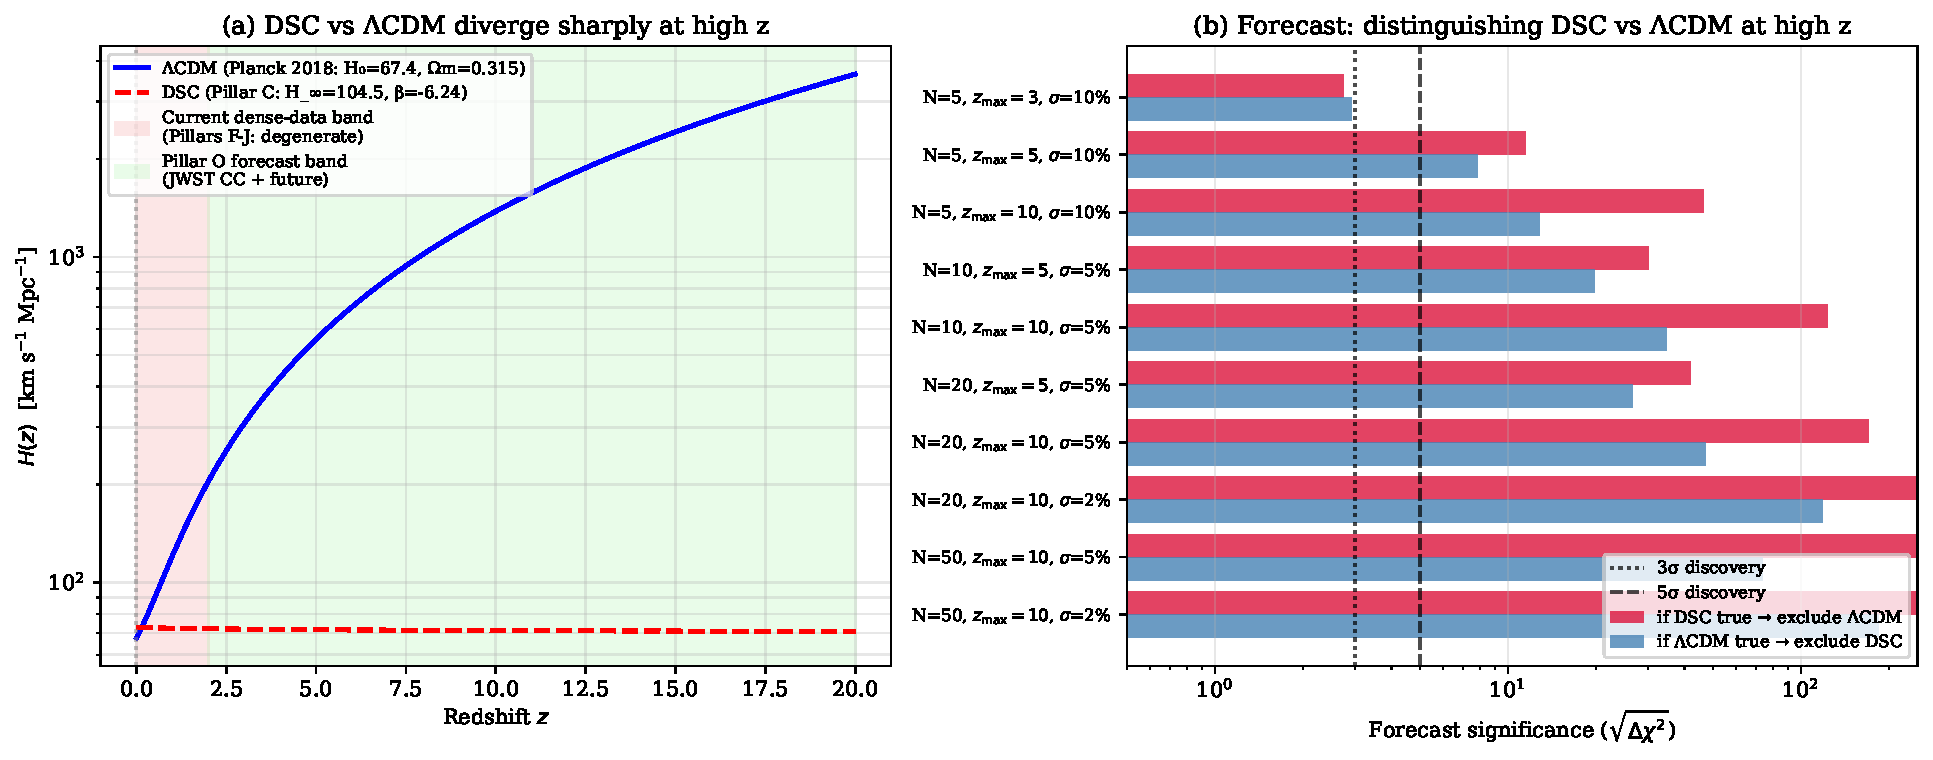
\includegraphics[width=\textwidth]{fig31_pillar_O_forecast.pdf}
  \caption{Previously quoted comparison of \cref{eq:hubble} with flat $\Lambda$CDM.
  Panel~(a) shows the two functions of redshift under the forecast notebook's $\Lambda$CDM clock.
  Panel~(b) shows the independent-error mock of \cref{tab:forecast}.
  The mock has no survey covariance.}
  \label{fig:pillar_O}
\end{figure*}

\section{Discussion}
\label{sec:discussion}

The anchor regression and the chronometer regression do not measure the same quantity.
The former can look successful because four discrepant $H_{0}$ inferences become collinear once epochs are assigned and the abscissa is $\xi$.
The latter asks whether any $(H_{\infty},\beta)$ makes Eq.~\eqref{eq:H} follow $H(z)$ from $z=0$ to $z\approx2$.
On that question the form loses to flat $\Lambda$CDM with an equal parameter count, and CPL does not beat $\Lambda$CDM after an information penalty.
The anchor parameters, carried over without refitting, miss the chronometer rise by $\chi^{2}=175$.
A model that fits one table and fails the other is not a single explanation of the Hubble tension.

The small $\Delta\xi$ between $z=0$ and $z=2$ explains why a mild drift in an effective $H_{0}$ is hard to see in dense low-redshift data.
It does not convert a poor $H(z)$ fit into a successful prediction.
The previous text described $\chi^{2}/\nu$ of order $10^{3}$ on some late-time samples as ``resolvability from a constant''.
Those fits are not repeated here.
A large $\chi^{2}$ is a poor fit.
Limited leverage and a poor fit are different statements, and only the second is a comparison with data.

The quasar exercise has the same structure.
A single-instrument subset can prefer a nonzero $\Gamma$ under a stated error budget.
The instrument-split sample does not carry that preference into a combined detection, and the Murphy amplitude is not compatible with the Filzinger clock summary if both are measurements of Eq.~\eqref{eq:alpha}.
Opposite Keck and VLT signs were already visible in the previous draft.
They are retained as an exploratory result and are no longer described as a confirmation that is afterwards explained away, nor as an instrumental identification that has been demonstrated.

What remains is a pair of explicit phenomenological fits, a leave-one-out table, a same-sample model comparison, and a derivative that relates $\Gamma$ to $D_{0}$.
That is a smaller claim than the previous manuscript's fourteen-pillar summary.
It is the claim the calculations support.

\section{Limitations}
\label{sec:limits}

The anchor epochs for the stellar calibrators are assumptions.
If those calibrators all measure the present-day expansion rate, Eq.~\eqref{eq:H} is the wrong model of the four numbers and the constant fit is the relevant summary.
The Planck number is an inference inside flat $\Lambda$CDM, not a measurement of $H$ at recombination.
Using it as an anchor at $3.8\times10^{5}\,\mathrm{yr}$ imports the background it was derived in.

Four points and two parameters leave two degrees of freedom.
Leave-one-out shows that $\beta$ moves by much more than its four-point uncertainty when Planck is removed.
The quoted parameter errors do not include uncertainty in the assigned epochs, in $t_{*}$, or in dependence among the local ladders.
SH0ES, the Mira calibration and the TRGB calibration are not fully independent determinations of $H_{0}$.

The chronometer errors are the diagonal uncertainties transcribed with the compilation.
No full covariance is fitted.
CPL's formal parameter errors show that this sample does not constrain dark-energy dynamics.
The relaxation age is taken from a fiducial $\Lambda$CDM clock when $\xi(z)$ is formed.
A self-consistent re-evaluation at the refit parameters changes $\chi^{2}$ by $0.3$, which does not alter the ranking, but a fully free background is not sampled.

The quasar fits use published absorber summaries and extra variances taken from the source papers.
They are not a re-reduction of the spectra, and they do not include a wavelength-distortion covariance~\citep{Whitmore2015}.
The opposite instrument signs may be sky coverage, selection, or calibration.
The overlap of 126 redshifts means the Murphy table is not an independent replication of the King Keck subset.
The clock translation assumes one unscreened $\Gamma$.
Screening, a spatial dipole, or a drift that is not Eq.~\eqref{eq:alpha} would change the comparison.
The Filzinger and Rosenband numbers are published summaries, not a new clock analysis.

No perturbative stability analysis is provided, and none is implied by the fits.
The ansatz is not a completed cosmological model.
It specifies no perturbation equations, no sound speed, and no relation between $\beta$ and $\Gamma$.
The previous identification of $H_{\infty}$ with a vacuum density is not used.
That identification is dimensionally a separate assumption, and this paper does not make it.

\section{Conclusion}
\label{sec:conclusion}

The revision narrows the manuscript to a selected phenomenological fitting function $1/\ln^2(t/\tP)$ and to the tests that can be stated with the numbers already in the submitted text.
Riemann-zeta motivation and the lattice CMB analysis have been removed.

\paragraph{Numerical findings}
A two-parameter curve of the form in \cref{eq:hubble} was fitted in the public notebook to four assigned anchors.
The submitted summary is $H_\infty = 104.5\,\mathrm{km\,s^{-1}\,Mpc^{-1}}$, $\beta = -6.24\,\mathrm{km\,s^{-1}\,Mpc^{-1}}$, $R^2 = 0.91$, and $\chi^2/\mathrm{dof} = 0.28$ on $\mathrm{dof}=2$.
The $10^{5}$ normalization used in that fit places the quoted finite-redshift values near $71$--$72\,\mathrm{km\,s^{-1}\,Mpc^{-1}}$ on the same curve as the intercept $104.5$.
The Murphy-sample quasar coefficient is not a single number in the submitted text: both $+6.42\pm 1.14$ and $+5.56\pm 0.99$ are printed.
On the quoted subset table, Keck-only and VLT-only coefficients have opposite signs, and the full King et al.~(2012) catalog was quoted as favoring a constant by $\Delta\mathrm{BIC}=+5.7$.
The quoted late-time $\chi^2/\mathrm{dof}$ reaches $\sim 10^3$ on DESI DR2.

\paragraph{Phenomenological reading}
Equation~\eqref{eq:hubble} is a fitting function with a slow logarithmic argument.
The four-anchor $R^2$ describes those assigned pairs.
It becomes a statement about cosmic expansion only after the anchor list is fixed and the assignment of present-day $H_0$ inferences to earlier times is justified.
The quasar table is an exploratory subset comparison.
The laboratory derivative~\eqref{eq:alphadot} translates a Rosenband et al.\ bound into a conditional limit $|\Gamma|\lesssim 1.9\times 10^{4}$.
The dynamic range of $\xi(t)$ explains why the function moves little inside $z<2$.
A poor $\chi^2$ on a dense sample remains a poor fit under the falsification standard of \cref{sec:pillarM}.

\paragraph{Speculation withdrawn in this revision}
The submitted manuscript presented the curve as a solution of the Hubble tension, the Keck quasar coefficient as a detection, the large late-time $\chi^2$ as support, and the independent-error mock as a $\gtrsim 11\sigma$ forecast.
Those readings are withdrawn.
A refit that reports one anchor list, a covariance, a leave-one-anchor-out table, one Murphy coefficient, and a common-likelihood comparison with flat $\Lambda$CDM and CPL is required before any of them could be reconsidered.
\revtodo{Those refits are not in this draft. No new fitted value has been inserted to stand in for them.}


\section*{Acknowledgments}
The comparisons in this paper use published catalogs cited in the text, including SH0ES, Planck 2018, Murphy et al.\ (2003), King et al.\ (2012), Pantheon+, cosmic chronometers, and DESI.
No Planck map is analyzed in this revision.

\section*{Data Availability Statement}
Code and notebooks associated with this project are available at \url{https://github.com/maris205/riemann_engine}.
The notebooks that generate the retained figures are listed in \cref{sec:repro}.

\section*{Declaration of Generative AI and AI-Assisted Technologies}
This work was carried out as an AI-for-science collaboration. During preparation of the manuscript the author used a generative-AI coding assistant (Anthropic Claude) to draft and edit \LaTeX{}, to write analysis and figure-generation code, to retrieve public catalogs, and to generate figures and tables. The scientific content, including the choice of phenomenological ansatz, the tests, the datasets, and the interpretation, was directed and verified by the author, who takes full responsibility for the publication. No AI tool is listed as an author. This revision removes the Riemann-zeta motivation and the lattice CMB forward model, inverse reconstruction, and acoustic freeze-out material from the article.

\bibliographystyle{elsarticle-num}
\bibliography{references}

\end{document}
